%\usepackage{beamerthemesplit}
%\usepackage[psamsfonts]{amsfonts}
%\usepackage{epsfig,graphicx,subfig,amsmath,amssymb,latexsym,stmaryrd,color,float}
\usepackage{epsfig,colordvi}
\usepackage{amsmath,amssymb,latexsym,stmaryrd}
\usepackage{float}
%\usepackage{algpseudocode}
%\usepackage{natbib}%[square,numbers]{natbib}
%\usepackage{threeparttable}
%\usepackage{multirow}
% Setup appearance:
\usepackage{multirow}

\setbeamertemplate{footline}[page number]
\usetheme{Raleigh}
%\usetheme{Antibes}
\usecolortheme{lily}
%\usetheme{Darmstadt}
%\usetheme{juanlespins}
%\usefonttheme[onlylarge]{structurebold}
\usefonttheme{professionalfonts}
\setbeamerfont*{frametitle}{size=\normalsize,series=\bfseries}
\setbeamertemplate{navigation symbols}{}


% Standard packages

\usepackage[english]{babel}
%\usepackage[latin2]{inputenc}
\usepackage{times}
\usepackage[T1]{fontenc}
\usepackage{textcomp}     % access \textquotesingle
%
% Setup TikZ
%
\usepackage{tikz}
\usetikzlibrary{arrows}
\tikzstyle{block}=[draw opacity=0.7,line width=1.4cm]

% the next line supposedly puts logo in bottom left
%\logo{\includegraphics[width=.1\textwidth]{buzz_hover}\hspace*{.88\paperwidth}}
% the next line puts logo in bottom right
\logo{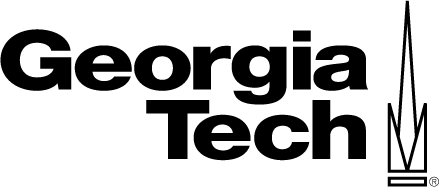
\includegraphics[width=.1\textwidth]{GT-Logo}}

\newcommand{\paws}{\pause}
\renewcommand{\paws}{}

\newcommand{\BC}{\begin{center}}
\newcommand{\EC}{\end{center}}
\newcommand{\BE}{\begin{equation}}
\newcommand{\EE}{\end{equation}}
\newcommand{\BEA}{\begin{eqnarray}}
\newcommand{\EEA}{\end{eqnarray}}
\newcommand{\BEAS}{\begin{eqnarray*}}
\newcommand{\EEAS}{\end{eqnarray*}}
\newcommand{\BEG}{\begin{example}\rm}
\newcommand{\EEG}{\end{example}}
\newcommand{\BTHM}{\begin{theorem}\rm}
\newcommand{\ETHM}{\end{theorem}}
\newcommand{\BCOR}{\begin{cor}\rm}
\newcommand{\ECOR}{\end{cor}}
\newcommand{\BPF}{\begin{proof}\rm}
\newcommand{\EPF}{\end{proof}}
\newcommand{\BRMK}{\begin{remark}\rm}
\newcommand{\ERMK}{\end{remark}}
\newcommand{\BLEM}{\begin{lemma}\rm}
\newcommand{\ELEM}{\end{lemma}}
\newcommand{\BIT}{\begin{itemize}}
\newcommand{\EIT}{\end{itemize}}
\newcommand{\DEF}{{\bfblue Definition}}
\newcommand{\RMK}{{\bfblue Remark}}
\newcommand{\RMKS}{{\bfblue Remarks}}
\newcommand{\THM}{{\bfblue Theorem}}
\newcommand{\COR}{{\bfblue Corollary}}
\newcommand{\PF}{{\bfblue Proof}}
\newcommand{\EG}{{\bfblue Example}}
\newcommand{\EGS}{{\bfblue Examples}}
\newcommand{\NOTN}{{\bfblue Notation}}


%\definecolor{myred}{HTML}{B3A369} % my tech gold from GT website
%\definecolor{myred}{HTML}{8E8B77} % Joe's tech gold
\definecolor{myred}{HTML}{EAAA00} % Joe's alternate gold
%\newcommand{\bfred}{\large \rm \color{myred}}
\newcommand{\bfred}{\bf \color{myred}}
%\newcommand{\bfred}{\color{red}}
%\definecolor{myblue}{HTML}{4277BB} % Joe's tech blue
\definecolor{myblue}{HTML}{003057} % Joe's alternate blue from GT website
%\newcommand{\bfblue}{\large \rm \color{myblue}}
\newcommand{\bfblue}{\bf \color{myblue}}
%\newcommand{\bfblue}{\color{blue}}
\newcommand{\myboldmath}{\boldmath} % turn this on if \bfred or \bfblue are actually using boldface (so that math symbol will also be in boldface}
%\newcommand{\myboldmath}{}

\newcommand{\dst}{\displaystyle}
\newcommand{\eq}{{\mbox{$\;\; = \;\;$}}}
\newcommand{\qbox}{{\mbox{\quad $\Box$}}}
\def\contradict
{
\tikz[baseline, x=0.2em, y=0.2em, line width=0.04em]
\draw (0,0) -- ({4*cos(45)},{4*sin(45)})
    (-1,1) -- ({-1 + 4*cos(45)},{1 + 4*sin(45)})
    (-1,3) -- ({-1 + 4*cos(315)},{3 + 4*sin(315)})
    (0,4) -- ({0 + 4*cos(315)},{4 + 4*sin(315)});
}
%
\newenvironment{proof2}[2][Proof of Theorem]{\textbf{#1 #2:} }{\hfill $\Box$} %{\ \ rule{0.5em}{0.5em}}
\newenvironment{proof3}[2][Proof of Theorems]{\textbf{#1 #2:} }{\hfill $\Box$} %{\ \ rule{0.5em}{0.5em}}
\newenvironment{assump}[1][Assumption]{\textbf{#1} }{\hfill $\Box$} %{\ \ rule{0.5em}{0.5em}}
%
\newcommand{\iid}{\mbox{$ \ \stackrel{\rm iid}{\sim} \ $}}
\newcommand{\bin}[2]{{{#1} \choose {#2}}}
\renewcommand{\Pr}{\mbox{$P$}} % Normal operator
\newcommand{\hs}[1]{\hspace{#1}}
\newcommand{\vs}[1]{\vspace{#1}}
\newcommand{\vsp}{\vspace{.1in}}
\newcommand{\ra}{\rightarrow}
\newcommand{\la}{\leftarrow}
\newcommand{\Ra}{\Rightarrow}
\newcommand{\RA}{\Longrightarrow}
\newcommand{\E}{\mathrm{E}} % expectation operator
\newcommand{\Var}{\mathrm{Var}} % Var operator
\newcommand{\Cov}{\mathrm{Cov}} % Cov operator
\newcommand{\Corr}{\mathrm{Corr}} % Corr operator
\newcommand{\Bias}{\mathrm{Bias}} % Bias operator
\newcommand{\MSE}{\mbox{MSE}} % MSE operator
\newcommand{\Nor}{\mbox{\rm Nor}} % Normal operator
\newcommand{\natlog}{\ell{\rm n}}
\newcommand{\bX}{\mbox{\bf X}}
\newcommand{\W}{\mathcal{W}} % stnd brown. motion operator
\newcommand{\B}{\mathcal{B}} % brown. bridge operator
\newcommand{\A}{\mathcal{A}}
\newcommand{\C}{\mathcal{C}}
\newcommand{\cid}{\mbox{$ \ \stackrel{d}{\longrightarrow} \ $}} % convergence in distribution
\newcommand{\ciD}{\mbox{$ \ \stackrel{\mathcal{D}}{\longrightarrow} \ $}} % convergence in distribution with D
\newcommand{\cip}{\mbox{$ \ \stackrel{p}{\longrightarrow} \ $}} % convergence in probability
\newcommand{\cas}{\mbox{$ \ \stackrel{a.s.}{\longrightarrow} \ $}} % almost sure (w.p. 1) convergence
\newcommand{\cm}{\mbox{$ \ \stackrel{L^1}{\longrightarrow} \ $}} % convergence in mean
\newcommand{\cqm}{\mbox{$ \ \stackrel{L^2}{\longrightarrow} \ $}} % convergence in quadradic mean
\newcommand{\zee}{\hbox{{\sf Z}\kern-.3550em\hbox{{\sf Z}}}} % set of natural numbers
\newcommand{\real}{\hbox{{I\kern-.1667em\hbox{R}}}} % set of real numbers
\newcommand{\BOX}{\rule[-2pt]{4pt}{8pt}}
\newcommand{\id}{\mathrm{d}} % d letter in integral
\renewcommand{\arraystretch}{1.25}
\definecolor{DB}{rgb}{0,0.08,0.45}
\definecolor{BB}{rgb}{0.1,0,0.35}
\definecolor{Bd}{rgb}{0.1,0,0.8}

\newcommand{\Simley}[1]{%
\begin{tikzpicture}[scale=0.11]
    \newcommand*{\SmileyRadius}{1.5}%
    \draw [fill=brown!10] (0,0) circle (\SmileyRadius)% outside circle
        %node [yshift=-0.22*\SmileyRadius cm] {\tiny #1}% uncomment this to see the smile factor
        ;

    \pgfmathsetmacro{\eyeX}{0.5*\SmileyRadius*cos(30)}
    \pgfmathsetmacro{\eyeY}{0.5*\SmileyRadius*sin(30)}
    \draw [fill=cyan,draw=none] (\eyeX,\eyeY) circle (0.15cm);
    \draw [fill=cyan,draw=none] (-\eyeX,\eyeY) circle (0.15cm);

    \pgfmathsetmacro{\xScale}{2*\eyeX/180}
    \pgfmathsetmacro{\yScale}{1.0*\eyeY}
    \draw[color=red, domain=-\eyeX:\eyeX]
        plot ({\x},{
            -0.1+#1*0.15 % shift the smiley as smile decreases
            -#1*1.75*\yScale*(sin((\x+\eyeX)/\xScale))-\eyeY});
\end{tikzpicture}%
}%

\newcommand{\SmallSimley}[1]{%
\begin{tikzpicture}[scale=0.11]
    \newcommand*{\SmileyRadius}{0.9}%
    \draw [fill=brown!10] (0,0) circle (\SmileyRadius)% outside circle
        %node [yshift=-0.22*\SmileyRadius cm] {\tiny #1}% uncomment this to see the smile factor
        ;

    \pgfmathsetmacro{\eyeX}{0.5*\SmileyRadius*cos(30)}
    \pgfmathsetmacro{\eyeY}{0.5*\SmileyRadius*sin(30)}
    \draw [fill=cyan,draw=none] (\eyeX,\eyeY) circle (0.15cm);
    \draw [fill=cyan,draw=none] (-\eyeX,\eyeY) circle (0.15cm);

    \pgfmathsetmacro{\xScale}{2*\eyeX/180}
    \pgfmathsetmacro{\yScale}{1.0*\eyeY}
    \draw[color=red, domain=-\eyeX:\eyeX]
        plot ({\x},{
            -0.1+#1*0.15 % shift the smiley as smile decreases
            -#1*1.75*\yScale*(sin((\x+\eyeX)/\xScale))-\eyeY});
\end{tikzpicture}%
}%

\def\double{\par\baselineskip=24pt}
\def\single{\par\baselineskip=12pt}
\def\oneandahalf{\par\baselineskip=18pt}

%\transboxin<1>
%\transglitter<2>
%\transwipe%<3>
%\transdissolve

\newcounter{lesson} 